\providecommand{\main}{..}
\documentclass[\main/main.tex]{subfiles}
\begin{document}
\chapter{Matching Covers}



\section{Matching}
\setlength\columnsep{25pt}
\begin{multicols}{2}
	\begin{definition}[Matching o Accoppiamento]
		Dato un grafo \(G=\rnd{V, E}\), un \textbf{matching} è un sottoinsieme \(M\subseteq E\) di archi \textit{a due a due non adiacenti}.
		\begin{figure}
			\NewAdigraph{MatchingDefinition}{
				1:2;
				2:2;
				3:2;
				4:2;
				5:2;
				6:2;
			}{
				1,2,red,2;
				3,4,red,2;
				5,+,gray;
			}[-]
			\MatchingDefinition{}
			\caption{Un esempio di matching, in rosso e grassetto.}
		\end{figure}
	\end{definition}
	\begin{definition}[Matching massimo]
		Matching \(M^*\) di cardinalità massima.
		\begin{figure}
			\NewAdigraph{MatchingDefinition}{
				1:2;
				2:2;
				3:2;
				4:2;
				5:2;
				6:2;
				7:2;
			}{
				1,2,red,2;
				3,4,red,2;
				5,6,red,2;
				5,+,gray;
			}[-]
			\MatchingDefinition{}
			\caption{Un esempio di matching massimo, in rosso e grassetto.}
		\end{figure}
	\end{definition}
	\begin{definition}[Matching bipartito]
		Se il grafo \(G\) è \textbf{bipartito}, allora anche \(M\) si dice \textbf{bipartito}.
		\begin{figure}
			\NewAdigraph{MatchingDefinition}{
				1:2;
				a:2;
				2:2;
				b:2;
				3:2;
				c:2;
			}{
				1,a,red,2;
				3,a,gray;
				2,b,red,2;
				2,c,gray;
				2,a,gray;
				3,c,gray;
			}[-]
			\MatchingDefinition{}
			\caption{Un esempio di matching bipartito, in rosso e grassetto.}
		\end{figure}
	\end{definition}
	\begin{definition}[Matching perfetto]
		Se la cardinalità del matching è pari a metà del numero di vertici, allora si dice \textbf{perfetto}:
		\[
			\abs{M} = \frac{\abs{V}}{2}
		\]
		\begin{figure}
			\NewAdigraph{MatchingDefinition}{
				1:2;
				2:2;
				3:2;
				4:2;
				5:2;
				6:2;
			}{
				1,2,red,2;
				3,4,red,2;
				5,6,red,2;
				5,+,gray;
			}[-]
			\MatchingDefinition{}
			\caption{Un esempio di matching perfetto, in rosso e grassetto}
		\end{figure}
	\end{definition}
\end{multicols}
\clearpage
\begin{definition}[Matching massimale]
	Un matching \(M\) si dice \textbf{massimale} se ogni elemento di \(E\setminus M\) è adiacente ad almeno un elemento di \(M\).

	Un matching massimale \textbf{non} necessariamente è massimo, mentre un matching massimo è sempre massimale.
	\begin{figure}
		\NewAdigraph{MaximalMatching}{
			5:0,0;
			1:2,2;
			3:2,-2;
			2:6,2;
			4:6,-2;
			6:8,0;
		}{
			5,1,gray;
			6,3,gray;
			3,4,gray;
			1,2,gray;
			2,6,gray;
			4,6,gray;
			3,1,red,2;
			4,2,red,2;
			2,3,gray;
			4,1,gray;
		}[-]
		\MaximalMatching{}
		\caption{Esempio di matching massimale, in rosso e grassetto}
	\end{figure}
\end{definition}
\clearpage
\section{Insieme stabile}
\begin{definition}[Insieme stabile o indipendente]
	Dato un grafo simmetrico \(G=\rnd{V, E}\), un qualunque sottoinsieme \(S\) di vertici si dice \textbf{indipendente} o \textbf{stabile} se esso è costituito da elementi \textit{a due a due non adiacenti}.
	\begin{figure}
		\NewAdigraph{InsiemeStabile}{
			1,red:0,4;
			2:4,4;
			3:0,0;
			4,red:4,0;
			5:1,3;
			6,red:3,3;
			7,red:1,1;
			8:3,1;
		}{
			1,2;
			1,3;
			1,5;
			2,6;
			2,4;
			4,8;
			4,3;
			3,7;
			5,6;
			5,7;
			6,8;
			7,8;
		}[-]
		\InsiemeStabile{}
		\caption{Esempio di insieme stabile}
	\end{figure}
\end{definition}
\begin{definition}[Insieme stabile massimo]
	Un insieme stabile \(S^*\) si dice \textbf{massimo} se \(\abs{S^*} \geq \abs{S}\), per ogni insieme stabile \(S\) di G.

	\begin{figure}
		\NewAdigraph{InsiemeStabile}{
			1:0,4;
			2,red,2:4,4;
			3,red,2:0,0;
			4:4,0;
			5,red,2:1,3;
			6:3,3;
			7:1,1;
			8,red,2:3,1;
		}{
			1,2;
			1,3;
			1,5;
			2,6;
			2,4;
			4,8;
			4,3;
			3,7;
			5,6;
			5,7;
			6,8;
			7,8;
		}[-]
		\InsiemeStabile{}
		\caption{Esempio di insieme stabile, in rosso e grassetto}
	\end{figure}
\end{definition}
\begin{definition}[Insieme stabile massimale]
	Un insieme stabile \(S\) si dice \textbf{massimale} se ogni elemento di \(V\setminus S\) è adiacente ad almeno un elemento di \(S\).

	\begin{figure}
		\NewAdigraph{InsiemeStabile}{
			1:0,4;
			2,red,2:4,4;
			3:0,0;
			4:4,0;
			5:1,3;
			6:3,3;
			7,red,2:1,1;
			8:3,1;
		}{
			1,2;
			1,3;
			1,5;
			2,6;
			2,4;
			4,8;
			4,3;
			3,7;
			5,6;
			5,7;
			6,8;
			7,8;
		}[-]
		\InsiemeStabile{}
		\caption{Esempio di insieme stabile, in rosso e grassetto}
	\end{figure}
\end{definition}
\clearpage
\section{Copertura}
\begin{definition}[Copertura]
	Dato un grafo simmetrico \(G = \rnd{V, E}\), un qualunque sottoinsieme \(T\) di vertici \textit{(\(F\) di archi)} tale che ogni arco di \(E\) \textit{(vertice di \(V\))} incide su almeno un elemento di \(T\) \textit{(di \(F\))} si dice \textbf{copertura}.

	In particolare, l'insieme \(T\) è detto \textbf{insieme trasversale} o \textbf{vertex cover} mentre l'insieme \(F\) è detto \textbf{edge cover}.
	\begin{figure}
		\begin{subfigure}{0.49\textwidth}
			\NewAdigraph{VertexCover}{
				1,red,2:2;
				2:2;
				3,red,2:2;
				4:2;
				5,red,2:2;
				6:2;
				7:2;
			}{
				1,2,gray;
				3,4,gray;
				5,6,gray;
				5,4,gray;
				5,7,gray;
				5,+,gray;
			}[-]
			\VertexCover{}
			\caption{Vertex cover, in rosso}
		\end{subfigure}
		\begin{subfigure}{0.49\textwidth}
			\NewAdigraph{EdgeCover}{
				1:2;
				2:2;
				3:2;
				4:2;
				5:2;
				6:2;
				7:2;
			}{
				1,2,red,2;
				3,4,red,2;
				5,6,red,2;
				5,7,red,2;
				5,+,gray;
			}[-]
			\EdgeCover{}
			\caption{Edge cover, in rosso}
		\end{subfigure}
		\caption{Esempi di edge e vertex cover}
	\end{figure}
\end{definition}
\begin{definition}[Copertura minima]
	Una copertura \(X^*\) si dice \textbf{minima} se:
	\[\abs{X^*} \leq \abs{X} \quad \forall X \in G\]
	Dove \(X\) sono gli insiemi di copertura del grafo \(G\).
\end{definition}
\begin{definition}[Copertura minimale]
	Una copertura \(X\) si dice \textbf{minimale} se \(X \setminus \crl{x}\) non è una copertura per ogni \(x \in X\).
\end{definition}
\clearpage
\section{Disuguaglianze duali deboli}
\begin{theorem}[Disuguaglianze duali deboli]
	\label{duali_deboli}
	Definiamo per un grafo \(G\):
	\begin{description}
		\item[\(\a(G)\)] la cardinalità dell'\textbf{insieme stabile massimo} del grafo \(G\).
		\item[\(\mu(G)\)] la cardinalità del \textbf{matching massimo} del grafo \(G\).
		\item[\(\rho(G)\)] la cardinalità dell'\textbf{edge cover minimo} di \(G\).
		\item[\(\tau(G)\)] la cardinalità dell'\textbf{insieme trasversale minimo} di \(G\).
	\end{description}

	Per un grafo \(G\) valgono le seguenti due disuguaglianze:
	\begin{align*}
		\a(G)  & \leq \rho(G) \\
		\mu(G) & \leq \tau(G)
	\end{align*}
	L'\textbf{insieme stabile minimo di un grafo} è sempre di cardinalità minore dell'\textbf{edge cover minimo}. Inoltre, l'\textbf{insieme stabile massimo} è sempre minore o uguale dell'\textbf{insieme trasversale minimo}.
\end{theorem}
\begin{proof}[Disuguaglianze duali deboli]
	Dato un grafo \(G=\rnd{V,E}\), ne definiamo un \textbf{insieme stabile} \(X\)  ed un \textbf{edge cover} \(Y\).

	Poiché \(Y\) è una \textit{edge cover}, ogni elemento di \(X\) incide su almeno un elemento di \(y\).

	Nessun elemento di \(Y\) copre contemporaneamente due elementi di \(X\), che altrimenti non sarebbe un \textit{insieme stabile}.

	Per ogni elemento di \(X\) esiste un distinto elemento di \(Y\) che lo copre, e quindi \(\abs{X} \leq \abs{Y}\), che per gli insiemi ottimi \(X^*\) e \(Y^*\) risulta:
	\[
		\a(G) \leq \rho(G)
	\]
	Ripetendo l'operazione con gli insiemi sui lati \(E\), si ottiene anche la seconda disequazione \(\mu(G) \leq \tau(G)\).
\end{proof}
\clearpage
\subsection{Diagramma della dimostrazione - Disuguaglianze duali deboli}
\begin{figure}
	\includegraphics[width=0.6\textwidth]{proofs/disdual}
\end{figure}
\clearpage
\section{Teorema di Gallai}
\begin{theorem}[Teorema di Gallai]
	Per ogni grafo \(G\) con \(n\) nodi si ha:
	\[
		\a(G) + \tau(G) = n
	\]
	Se inoltre \(G\) non ha nodi isolati
	\[
		\mu(G) + \rho(G) = n
	\]
	Cioè la somma della cardinalità di \textbf{insieme stabile massimo} e \textbf{insieme trasversale minimo} di un grafo \(G\) sono pari al numero dei suoi nodi.

	Se non esistono nodi isolati, la stessa relazione vale anche per la somma della cardinalità del \textbf{matching massimo} e dell'\textbf{edge cover minimo} di un grafo \(G\).
\end{theorem}
\begin{proof}[Teorema di Gallai]
	\textit{Iniziamo ottenendo la prima equazione:} sia \(S\) un \textbf{insieme stabile} di \(G\). Allora \(V\setminus S\) è un \textbf{insieme trasversale}.

	In particolare, vale che \(\abs{V\setminus S} \geq \tau(G)\).

	Se consideriamo l'insieme stabile massimo \(S^*\), otteniamo:
	\[
		\tau(G) \leq \abs{V\setminus S^*} = n - \a(G) \quad \Rightarrow \quad \a(G) + \tau(G) \leq n
	\]
	Analogamente, sia \(T\) un \textbf{insieme trasversale} di \(G\). Allora \(V\setminus T\) è un \textbf{insieme stabile}.

	In particolare, \(\abs{V-T} \leq \a(G)\).

	Se consideriamo l'insieme trasversale minimo \(T^*\), otteniamo:
	\[
		\a(G) \geq \abs{V\setminus T^*} = n - \tau(G) \quad \Rightarrow \quad \a(G) + \tau(G) \geq n
	\]
	Per le due disequazioni ottenute possiamo affermare che:
	\[
		\a(G) + \tau(G) \leq n \quad \land \quad \a(G) + \tau(G) \geq n \quad \Rightarrow \quad \a(G) + \tau(G) = n
	\]
	\textit{Procediamo a dimostrare la seconda equazione:} sia \(G\) un grafo privo di nodi isolati e sia \(M^*\) il \textbf{matching massimo} di \(G\). Indichiamo con \(V_{M^*}\) i nodi che sono estremi degli archi in \(M^*\).

	Sia \(H\) un \textbf{insieme minimale} di archi tale che ogni nodo in \(V\setminus V_{M^*}\) è estremo di qualche arco in \(H\). Segue che:
	\[
		\abs{H} = \abs{V\setminus V_{M^*}} = n - 2\abs{M^*}
	\]
	Osserviamo che l'insieme \(C=H\cup M^*\) è un edge-cover di \(G\). Sicuramente, \(\abs{C} \geq \rho(G)\), quindi:
	\[
		\rho(G) \leq \abs{C} = \abs{M^*} + \abs{H} = \abs{M^*} + n - 2\abs{M^*} = n - \abs{M^*} = n - \mu(G) \quad \Rightarrow \quad \rho(G) + \mu(G) \leq n
	\]
	Sia \(C^*\) il \textbf{minimo edge-cover} su \(G\), cioè tale che \(\abs{C^*} = \rho(G)\) e sia \(K = (V, C^*)\) il sottografo indotto da \(C^*\). Valgono quindi le seguenti proprietà:

	\begin{enumerate}
		\item \(K\) è un grafo aciclico.
		\item Ogni cammino di \(K\) è composto al più da due archi.
		\item \(K\) possiede \(\abs{V} = n\) vertici.
		\item \(K\) possiede \(\abs{C^*} = \rho(G)\) lati.
		\item \(K\) può essere decomposto in \(N\) componenti connesse aventi la forma di stella.
	\end{enumerate}

	Consideriamo l'\(i\)-esima componente connessa di \(K\) e ne indichiamo con \(s_i\) il numero di nodi mentre con \(s_i-1\) il numero di archi:
	\[
		n = \sum_{i=1}^N s_i \quad \text{e} \quad \rho(G) = \sum_{i=1}^N (s_i -1) = n - N \Rightarrow N = n - \rho(G)
	\]
	Sia \(M\) un matching con un arco per ogni componente di \(K\). Si ottiene:
	\[
		\mu(G) \geq \abs{M} = n - \rho(G) \Rightarrow \rho(G) + \mu(G) \geq n
	\]
	Possiamo quindi concludere che:
	\[
		\rho(G) + \mu(G) \leq n \quad \land \quad \rho(G) + \mu(G) \geq n\quad \Rightarrow \quad\rho(G) + \mu(G) = n
	\]

\end{proof}
\clearpage
\subsection{Diagramma della dimostrazione - Teorema di Gallai}
\begin{figure}
	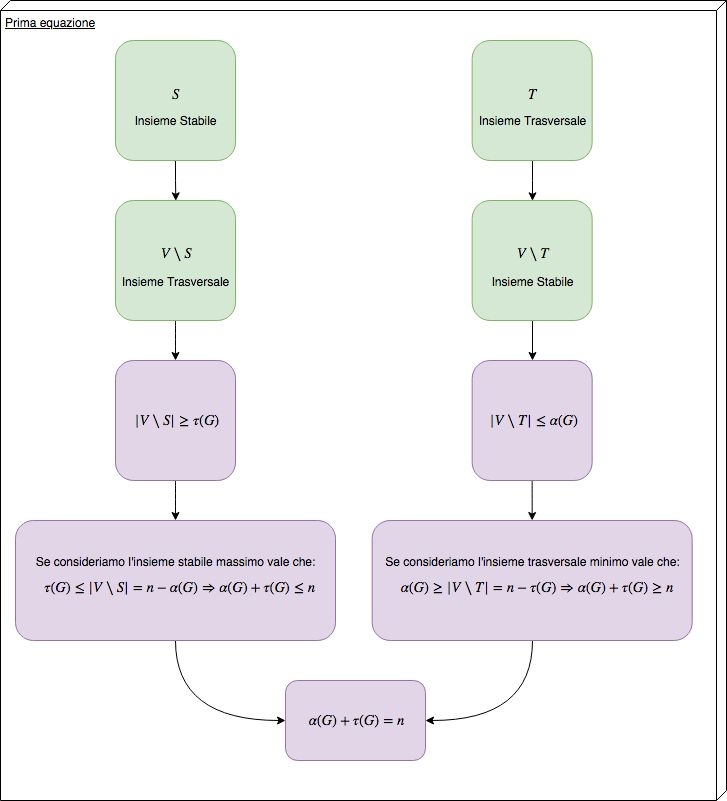
\includegraphics[width=\textwidth]{proofs/Gallai1}
\end{figure}
\clearpage
\begin{figure}
	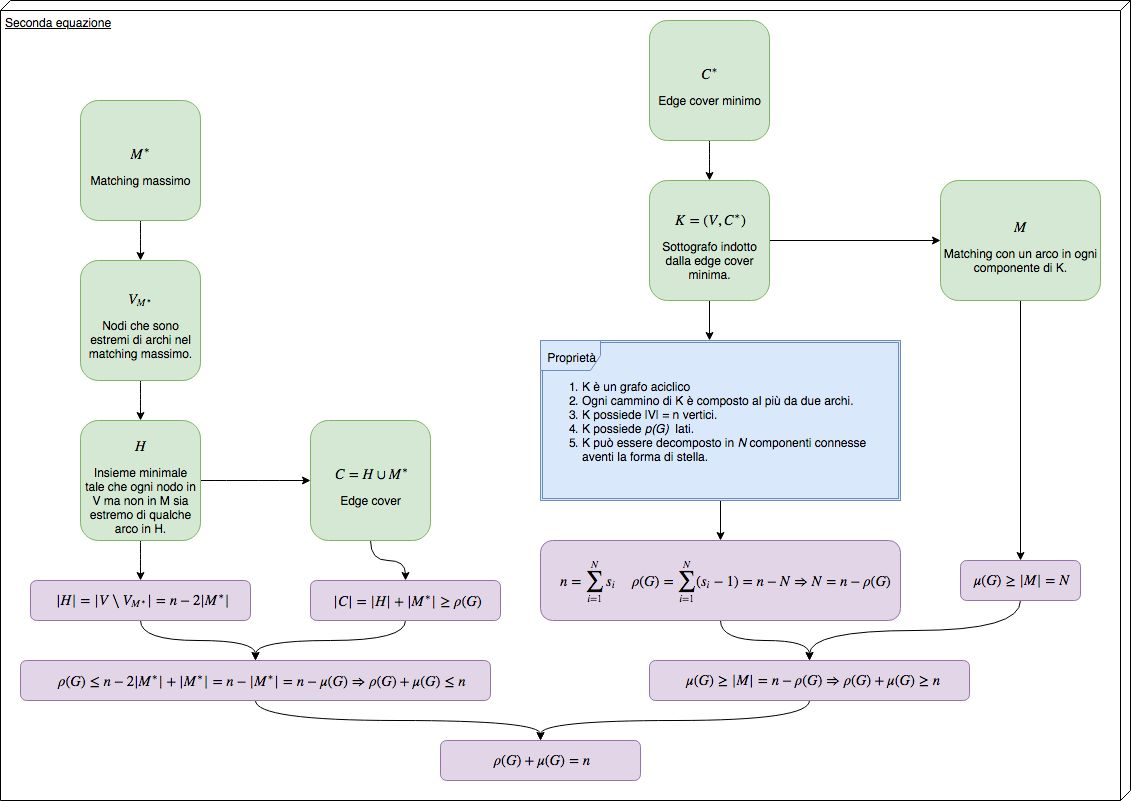
\includegraphics[width=\textwidth]{proofs/Gallai2}
\end{figure}
\clearpage
\section{Cammino alternante e aumentante}
\begin{multicols}{2}[Sia \(M\) un matching di \(G = \rnd{V, E}\).]
	\begin{definition}[Arco accoppiato]
		Un arco \(\rnd{i,j} \in E\) si dice \textbf{accoppiato} se:
		\[
			\rnd{i,j} \in M
		\]
		Altrimenti è detto \textbf{libero}.
	\end{definition}
	\begin{definition}[Vertice accoppiato]
		Un vertice \(i \in V\) si dice \textbf{accoppiato} se su di esso incide un arco di \(M\). Altrimenti si dice che \textbf{non incide}.
	\end{definition}
	\begin{definition}[Cammino alternante]
		Un cammino \(P\) sul grafo \(G\) si dice \textbf{alternante} rispetto a \(M\) se esso è costituito alternativamente da archi accoppiati e liberi.
	\end{definition}
	\begin{definition}[Cammino aumentante]
		Un cammino \(P\) \textit{alternante} rispetto ad \(M\) che abbia entrambi gli estremi esposti si dice \textbf{aumentante}.
	\end{definition}
\end{multicols}

\begin{theorem}[Estensione di un Matching tramite un cammino aumentante]
	Sia \(M\) un matching definito sul grafo \(G\) e sia \(P\) un cammino aumentante rispetto a \(M\).

	La \textbf{differenza simmetrica}:
	\[
		M' = \rnd{M\setminus P} \cup \rnd{P\setminus M} = M \oplus P = M \Delta P
	\]
	È un \textbf{matching} di \textbf{cardinalità} \(\abs{M} + 1\).
\end{theorem}

\begin{proof}[Estensione di un Matching tramite un cammino aumentante]
	Dimostriamo che l'insieme \(M'\) definito tramite \textbf{diiffenza simmetrica} gode delle due proprietà descritte:
	\begin{description}
		\item \textbf{\(M'\) è un matching:}
		      \begin{description}
			      \item[\(\forall v \in \rnd{M \setminus P}\)] Per i nodi che non sono toccati da \(P\) non è cambiato nulla: su di essi incide un solo arco di \(M\) che ora appartiene anche ad \(M'\).
			      \item[\(\forall v \in \rnd{P \setminus M}: v\neq v_s \land v \neq v_t\)] Sui nodi intermedi di \(P\) incide soltanto un arco di \(P\setminus M\), e quindi di \(M'\).
			      \item[\(\forall v \in \rnd{P \setminus M}: v= v_s \lor v = v_t\)] I nodi estremi di \(P\) prima erano esposti mentre ora sono accoppiati e su di essi incide soltanto un arco di \(P\setminus M\).
		      \end{description}
		\item \textbf{\(M'\) ha un elemento in più di \(M\):}
		      \begin{enumerate}
			      \item Sia \(\abs{M} = m_1 + m_2\) con \(m_1 = \text{``Archi unicamente di \(M\)''}\) ed \(m_2 = \text{Archi condivisi tra il matching \(M\) ed il cammino \(P\)}\).
			      \item Poiché \(P\) è aumentante, \(\abs{P} = m_2 + \rnd{m_2 + 1}\) dove \(m_2 + 1 = \abs{P\setminus M}\).
			      \item \(\abs{M'} = \abs{M \setminus P} + \abs{P \setminus M} = m_1 + m_2 + 1 = \abs{M} +1\)
		      \end{enumerate}
	\end{description}
\end{proof}
\clearpage
\subsection{Diagramma della dimostrazione - Estensione di un Matching tramite un cammino aumentante}
\begin{figure}
	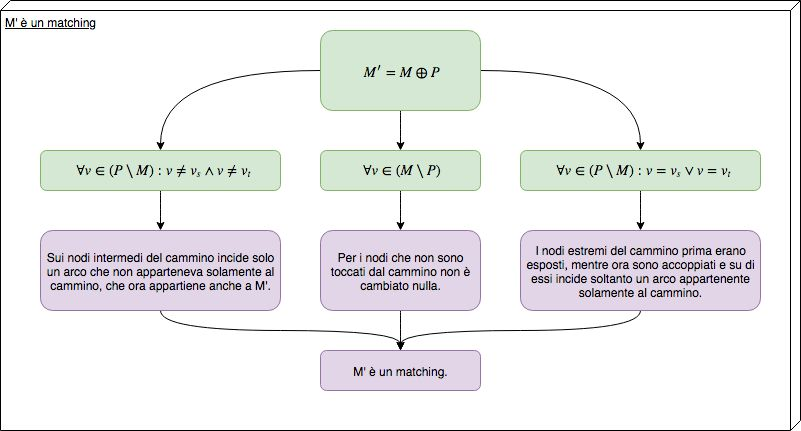
\includegraphics[width=\textwidth]{proofs/Estensione1}
\end{figure}
\begin{figure}
	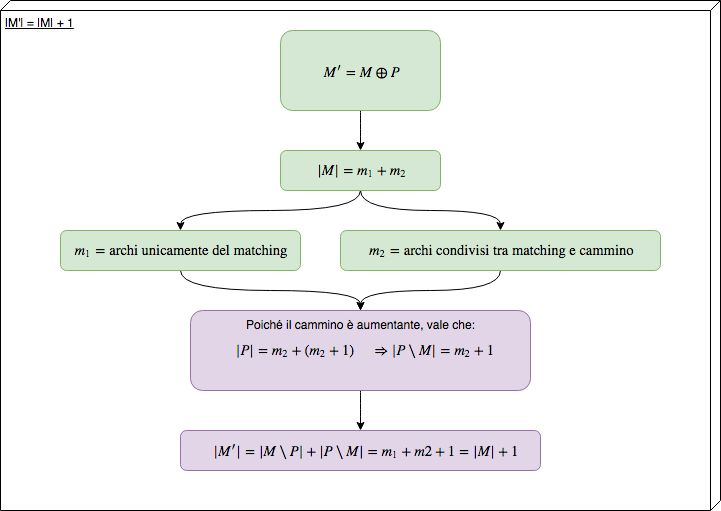
\includegraphics[width=\textwidth]{proofs/Estensione2}
\end{figure}
\clearpage
\begin{theorem}[Teorema di Berge]
	Un matching \(M\) di \(G\) è massimo \textbf{se e solo se} \(G\) non ammette cammini aumentanti rispetto a \(M\).
\end{theorem}
\begin{proof}[Teorema di Berge]
	La condizione sufficiente segue dal teorema precedente. Procediamo quindi a dimostrare la condizione necessaria.

	Supponiamo che \(G\) ammetta un matching \(M'\) con un elemento in più di \(M\). Mostriamo che allora esiste un cammino aumentante per \(M\).

	Consideriamo l'insieme di archi:
	\[
		F = \rnd{M'\cup M}\setminus\rnd{M' \cap M}
	\]
	e sia \(G' \subseteq G\) con \(E' = F\).

	Analizziamo il grado di ciascun \(v \in V'\), considerando tutti i casi possibili:
	\begin{enumerate}
		\item Un nodo su cui incide lo stesso arco appartenente sia ad \(M\) che ad \(M'\) è un nodo isolato su \(G'\) e quindi ha grado \(0\).
		\item Un nodo su cui incide sia un arco di \(M\) sia un arco di \(M'\) è un nodo che ha grado \(2\) su \(G'\).
		\item Un nodo su cui incide un arco di \(M\) e nessun arco di \(M'\) o viceversa è un nodo che ha grado \(1\) su \(G'\).
		\item Un nodo esposto sia rispetto ad \(M\) che rispetto ad \(M'\) è un nodo isolato su \(G'\) e quindi ha grado \(0\).
	\end{enumerate}
	Pertanto in \(G'\) nessun nodo ha un grado superiore a 2 e possiamo concludere che le componenti connesse di \(G'\) sono o nodi isolati o percorsi o cicli.

	Nessun ciclo può essere dispari altrimenti ci sarebbero due archi dello stesso matching incidenti sullo stesso nodo e questo è impossibile.

	Non possono essere tutti cicli pari altrimenti \(\abs{M} = \abs{M'}\). Deve esistere una componente connessa che è un percorso.

	Non tutti i percorsi possono essere pari altrimenti, nuovamente, \(\abs{M} = \abs{M'}\).

	Quindi, senza perdita di generalità, possiamo assumere che esista un percorso dispari che inizia e termina con un arco di \(M'\).

	\textbf{Questo percorso è aumentante per \(M\).}
\end{proof}
\clearpage
\subsection{Diagramma della dimostrazione - Teorema di Berge}
\begin{figure}
	\includegraphics[width=0.75\textwidth]{proofs/Teorema_di_Berge}
\end{figure}
\clearpage
\section{Teorema del cammino aumentante}

\begin{theorem}[Teorema del cammino aumentante]
	Sia \(v\) un vertice esposto in un matching \(M\). Se non esiste un cammino aumentante per \(M\) che parte da \(v\), allora esiste un matching massimo avente \(v\) esposto.
\end{theorem}

\begin{proof}[Teorema del cammino aumentante]
	Sia \(M^*\) un matching massimo in cui \(v\) è accoppiato. Consideriamo \(\rnd{M^*\cup M}\setminus\rnd{M^* \cap M}\): questo insieme non può contenere un cammino alternante con i vertici degli archi di \(M\) esposti, altrimenti sarebbe aumentante per esso.

	Deve però contenere un cammino composto dallo stesso numero di archi dei due insiemi, \(M\) e \(M^*\): un cammino con un solo arco di un insieme, infatti, sarebbe aumentante per l'altro e viceversa.

	Consideriamo quindi un cammino \(P\) composto da un ugual numero di archi dai due insiemi e consideriamo un nuovo matching \(M' = \rnd{M^*\cup P}\setminus\rnd{M^* \cap P}\). Vanno osservate due proprietà:

	\begin{enumerate}
		\item La cardinalità del nuovo insieme e del matching massimo sono uguali:
		      \[
			      \abs{M'} = \abs{M^*}
		      \]
		\item Il nodo \(v\) è esposto rispetto ad \(M'\).
	\end{enumerate}
	Pertanto abbiamo individuato un nuovo matching massimo con \(v\) esposto.
\end{proof}
\clearpage
\subsection{Diagramma della dimostrazione - Teorema del cammino aumentante}
\begin{figure}
	\includegraphics[width=\textwidth]{proofs/Teorema_del_Cammino_Aumentante}
\end{figure}
\clearpage
\section{Teorema di König}

\begin{theorem}[Teorema di König]
	Se \(G=\rnd{X, Y, E}\) è un grafo bipartito, allora \(\mu(G) = \tau(G)\).
\end{theorem}

\begin{proof}[Teorema di König]
	Sia \(M^*\) un matching massimo, e siano:
	\begin{enumerate}
		\item \(X_1\) un insieme dei nodi \(x\) di \(X\) \textbf{accoppiati} rispetto ad \(M^*\)
		\item \(X_2\) un insieme dei nodi \(x\) di \(X\) \textbf{esposti} rispetto ad \(M^*\)
		\item \(Y_1\) insieme dei nodi \(y\) di \(Y\) raggiungibili da \(x\) in \(X_2\). Questi nodi, per definizione, sono \textbf{accoppiati} altrimenti \(M^*\) non sarebbe massimo.
		\item \(Y_2 = Y \setminus Y_1\)
	\end{enumerate}

	\begin{center}
		\begin{minipage}{0.618\textwidth}
			\begin{definition}[Nodo raggiungibile]
				Un nodo \(y \in Y\) è raggiungibile se esiste \(P\) alternante rispetto ad \(M^*\) da \(x\) in \(X_2\) tale che l'ultimo arco non appartiene ad \(M^*\).
			\end{definition}
		\end{minipage}
	\end{center}

	Consideriamo un set di nodi \(Z\) definito come:
	\[
		Z = \crl{z_1, z_2, \ldots, z_{\mu(G)}} \quad \text{con} \quad \begin{cases}
			z_i = y_i & \text{se \(y_i\) è raggiungibile} \\
			z_i = x_i & \text{altrimenti}
		\end{cases}
	\]
	\textbf{Procediamo ora a dimostrare che il set \(Z\) è \textit{trasversale}}.

	Iniziamo dimostrando che non esistono archi da nodi in \(X_2\) verso nodi in \(Y\) non coperti da \(Z\):

	\begin{enumerate}
		\item Non può esistere un arco non coperto da \(Z\) tra un nodo in \(X_2\) e un nodo in \(Y_2\), altrimenti il matching non sarebbe massimo.
		\item Non può esistere un arco non coperto da \(Z\) tra un nodo in \(X_2\) e un nodo in \(Y_1\) perché i nodi in \(Y_1\) sono raggiungibili e quindi l'arco necessariamente deve essere coperto.
	\end{enumerate}

	Dimostriamo ora che non esistono archi da nodi in \(X_1\) verso nodi in \(Y\) non coperti da \(Z\):

	Consideriamo un arco da \(X_1\) a \(Y_2\): se non fosse coperto, allora esisterebbe un nodo, estremo dell'arco del matching, raggiungibile da \(X_2\) in \(Y_2\). Ciò implicherebbe l'esistenza di un cammino aumentante ed il matching sarebbe pertanto non massimo.

	Consideriamo ora un arco da \(X_1\) a \(Y_1\): se il nodo terminale non fosse coperto non sarebbe raggiungibile (per la definizione di \(Y_1\) e di \(Z\)) e non apparterrebbe in primo luogo a \(Y_1\), quindi l'arco non esisterebbe.

	Pertanto, \(Z\) è un insieme trasversale di cardinalità pari a \(\mu(G)\).
\end{proof}
\clearpage
\begin{proof}[Teorema di König (Rizzi, 1999)]
	Dato un grafo \(G\), per le disuguaglianze duali deboli (\ref{duali_deboli}), vale che: \(\mu(G) \leq \tau(G)\). Per assurdo ipotizziamo che esistano grafi \textbf{bipartiti} per cui valga: \(\mu(G) < \tau(G)\).

	Tra tutti i possibili grafi che violano il teorema di König ne scegliamo uno come controesempio \textbf{minimo} (\textit{significa che qualsiasi grafo più piccolo andrebbe a rispettare il teorema di König}):
	\begin{enumerate}
		\item Il grafo \(G\) ha il più piccolo numero di vertici \(n\).
		\item Il grafo \(G\), tra tutti i possibili controesempi con \(n\) vertici, ha anche il numero minimo di lati.
	\end{enumerate}

	Ne segue che:

	\begin{enumerate}
		\item Il grafo \(G\) è \textbf{connesso}.
		\item Il grafo \(G\) non è composto da un \textbf{ciclo pari} (cicli di lunghezza dispari non sono possibili in un grafo bipartito) o un \textbf{cammino}, poiché grafi di questo genere chiaramente rispetterebbero il teorema di König.
	\end{enumerate}

	Ne segue che \(G\) ha un nodo \(u\) di grado almeno \(3\). Sia \(v\) uno dei nodi vicini di \(u\). Sia \(M^*_G\) il matching massimo per il grafo e \(M^*_{G\setminus v}\) il matching massimo per il grafo privato del nodo \(v\).

	\textit{NB: non è possibile costruire veramente il grafo G siccome stiamo procedendo per assurdo. L'immagine seguente serve per aiutare a visualizzare il procedimento, ma non è una reale rappresentazione del controesempio minimo \(G\).}

	\begin{figure}
		\begin{subfigure}{0.33\textwidth}
			\NewAdigraph{MinimalGraph}{
				u,red:0,0:$u$;
				p,blue:2:$p$;
				s,red:2:$s$;
				q,blue:2:$q$;
				t,red:2:$t$;
				v,blue:2:$v$;
				r,red:2:$r$;
			}{
				u,v;
				u,q:1:$f$;
				u,p;
				t,v,gray;
				r,p,gray;
				s,q,gray;
			}[-]
			\MinimalGraph{}
			\caption{Componente a stella di \(G\).}
		\end{subfigure}
		\begin{subfigure}{0.33\textwidth}
			\NewAdigraph{MinimalGraph}{
				u,red:0,0:$u$;
				p,blue:2:$p$;
				s,red:2:$s$;
				q,blue:2:$q$;
				t,red:2:$t$;
				v,blue:2:$v$;
				r,red:2:$r$;
			}{
				u,v,gray;
				u,q,gray:1:$f$;
				u,p,red,2;
				t,v,red,2;
				r,p,gray;
				s,q,red,2;
			}[-]
			\MinimalGraph{}
			\caption{Matching \(M^*_G\), in rosso.}
		\end{subfigure}
		\begin{subfigure}{0.33\textwidth}
			\NewAdigraph{MinimalGraph}{
				u,red:0,0:$u$;
				p,blue:2:$p$;
				s,red:2:$s$;
				q,blue:2:$q$;
				t,red:2:$t$;
				v,blue:2:$\xcancel{v}$;
				r,red:2:$r$;
			}{
				u,q,gray:1:$f$;
				u,p,red,2;
				r,p,gray;
				s,q,red,2;
			}[-]
			\MinimalGraph{}
			\caption{Matching \(M^*_{G\setminus v}\), in rosso.}
		\end{subfigure}
		\caption{Matching massimi e componente a stella.}
	\end{figure}
	Siccome \(G\) è stato scelto come un \textbf{controesempio minimo}, il grafo \(G\setminus v\) soddisfa il teorema di König (cioè modificando il grafo togliendo elementi si deve rientrare in un grafo che riespetta il teorema): \(\mu(G\setminus v) = \tau(G\setminus v)\). Procediamo quindi \textbf{assumendo} che \(\mu(G\setminus v)<\mu(G)\).

	Allora possiamo realizzare una vertex cover \(C_{G\setminus v}\) di cardinalità \(\mu(G\setminus v)\) ed estenderla ad essere una cover di \(G\) aggiungendovi il vertice \(v\): \(C_{G} = C_{G\setminus v} \cup \crl{v}\). Questo implica che:
	\[
		\tau(G) \leq \mu(G\setminus v) + 1 \leq \mu(G) \quad \Rightarrow \quad  \tau(G) = \mu(G)
	\]
	\textit{Pertanto \(G\) rispetterebbe il teorema di König, una contraddizione con l'ipotesi iniziale per cui \(\mu(G\setminus v)<\mu(G)\)}. Ne segue che \(\mu(G\setminus v) = \mu(G)\): deve esistere quindi un matching massimo \(M^*_G\) di \(G\) in cui nessun lato è incidente con \(v\).

	Siccome il nodo \(u\) possiede grado almeno pari a \(3\), possiamo scegliere un lato \(f=\rnd{u,q}: f \not\in M_G\). Nuovamente per \textbf{minimalità} il nuovo grafo \(G\setminus f\) soddisfa il teorema di König ed è possibile ottenere:
	\[\mu(G) = \mu(G\setminus f) = \tau(G\setminus f)\]
	Sia \(C_{G\setminus f}\) una \textbf{vertex cover} con cardinalità pari a \(\mu(G)\): siccome nessun lato del matching \(M^*_G\) è incidente con \(v\), allora non sarà incluso nemmeno nella cover: \(v \not\in C_{G\setminus f}\).

	Questo avviene perché la cardinalità della cover \(C_{G\setminus f}\) e del matching \(M^*_G\) sono uguali ed un estremo di ogni lato del matching deve essere incluso nella cover.

	Ne segue che la cover \(C_{G\setminus f}\), per coprire il lato \(\rnd{u,v} \neq f\), deve includere l'altro estremo \(u\), e risulta pertanto essere una vertex cover per \(G\).

	Per cui, nuovamente, risulta che \(G\) soddisfi il teorema di König: questa ultima contraddizione conferma la validità del teorema.
\end{proof}
\clearpage
\subsection{Diagramma della dimostrazione - Teorema di König (Rizzi, 1999)}
\begin{figure}
	\includegraphics[width=\textwidth]{proofs/Teorema_di_König,_Rizzi}
\end{figure}
\clearpage
\section{Teorema di Hall o dei matrimoni}
\begin{theorem}[Teorema di Hall]
	Sia \(G = \rnd{V_1 \cup V_2, E}\) un grafo bipartito con \(\abs{V_1} \geq \abs{V_2}\). Dato un insieme di vertici \(J \subseteq V_2\), sia \(\Gamma(J) \) il set dei vertici in \(V_1\) che sono adiacenti a qualche vertice in \(J\). Allora:
	\[
		G \text{ ammette un \textbf{matching completo} } \Leftrightarrow \abs{\Gamma(J)} \geq \abs{J} \quad \forall J \subseteq V_2
	\]
	Cioè in un \textbf{grafo bipartito} esiste un \textbf{matching completo} se e solo se ogni vertice della componente minore ha almeno un vertice incidente distinto della componente maggiore.
\end{theorem}

\begin{proof}[Teorema di Hall]
	Sia \(M^*\) un \textbf{matching massimo} di \(G\) e \(J\) un sottoinsieme qualsiasi di \(V_2\). Sia \(E(J)\) l'insieme dei lati contenuti nel matching \(M^*\) che sono incidenti con un vertice in \(J\). Allora, i vertici terminali dei lati in \(E(J)\) che sono contenuti in \(V_1\) formano un sottoinsieme di cardinalità \(\abs{J}\) di \(\Gamma(J)\).

	Per assurdo, supponiamo che la condizione \(\abs{\Gamma(J)} \geq \abs{J}\) è valida e che non esista un matching completo \(\abs{M_G^*} < \abs{V_2}\). Allora per il \textbf{Teorema di König} è possibile costruire una \textbf{vertex cover} di tutti i lati con cardinalità \(\abs{X} = \abs{M_G^*} = \mu(G) < \abs{V_2}\):
	\[
		X=V'_1 \cup V'_2: V'_1 \subseteq V_1,\;V'_2 \subseteq V_2 \quad \abs{X} = \abs{V_1'} + \abs{V_2'} < \abs{V_2} \Rightarrow \abs{V'_1} < \abs{V_2} - \abs{V'_2} = \abs{V_2 \setminus V'_2}
	\]
	Sia ora \(v \in V_2 \setminus V'_2 \Rightarrow \Gamma(v) \subseteq V'_1\), poiché i lati incidenti a \(v\) devono esere coperti da qualche nodo \(\neq v\), quindi:
	\[
		\abs{\Gamma(V_2\setminus V'_2)} \geq \abs{V_2\setminus V'_2} \quad \land \quad \abs{\Gamma(V_2\setminus V'_2)} \leq \abs{V'_1} <  \abs{V_2\setminus V'_2}
	\]
	da cui la contraddizione.
\end{proof}
\clearpage
\subsection{Diagramma della dimostrazione - Teorema di Hall}
\begin{figure}
	\includegraphics[width=0.8\textwidth]{proofs/Teorema_di_Hall}
\end{figure}
\section{Formula di Tutte-Berge e Teorema di Tutte}
\subsection{Formula di Tutte-Berge}
\begin{theorem}[Formula di Tutte-Berge]
	La dimensione di un matching massimo in un grafo \(\Gr \) è pari a:
	\[
		\frac{1}{2} \min_{U \subseteq V} \crl{\abs{U} - \text{odd}\rnd{G\setminus U} + \abs{V}}
	\]
	dove \(\text{odd}(H)\) è il numero di componenti connesse del grafo \(H\) con un numero dispari di vertici.
\end{theorem}

Questa formula implica immediatamente una condizione per l'esistenza di un matching perfetto: il Teorema di Tutte.

\subsection{Teorema di Tutte}
\begin{theorem}[Teorema di Tutte]
	Un grafo \(\Gr \) contiene un matching perfetto se e solo vale che:
	\[
		\text{odd}\rnd{G\setminus A} \leq \abs{A} \quad \forall A \subseteq V
	\]
\end{theorem}
\clearpage
\section{Proposizioni sugli alberi alternanti}
\begin{definition}[Albero alternante]
	Un albero alternante è costruito a partire da un matching \(M\) di un grafo \(\Gr \) ed un nodo \(r \in V\) di \(M\) esposto.

	Costruiamo iterativamente set di nodi \(A\) e \(B\), in modo tale che ogni nodo \(A\) sia al termine di un cammino alternante di \(M\) di lunghezza dispari che inizia con \(r\), mentre ogni nodo \(B\) al termine di quelli pari.

	Tali insiemi possono essere costruiti iniziando da \(A=\emptyset, B=\crl{r}\) e seguendo la regola seguente:
	\[
		\rnd{v,w} \in E, v \in B, w \not\in A \cup B, \rnd{w,z} \in M \Rightarrow A' = A \cup \crl{w}, B' = B \cup \crl{z}
	\]

	L'albero così costruito possiede due proprietà:
	\begin{enumerate}
		\item Ogni nodo dell'albero oltre alla radice è coperto da un lato di \(M \cap E(T)\).
		\item Per ogni nodo \(v\) dell'albero, il cammino nell'albero da \(v\) alla radice è alternante nel matching \(M\) associato all'albero.
	\end{enumerate}

	Tali insiemi sono importanti poiché se identifichiamo un lato \(\rnd{v, w}\) tale che \(v \in B\) e \(w \not\in A \cup B\) ed esposto, allora esiste un cammino \(M\)-alternante da \(r\) a \(v\) che assieme a \(\rnd{v, w}\) va a formare un cammino \(M\)-aumentante.
\end{definition}
\begin{definition}[Estendere un albero alternante]
	\textbf{Input:} Un matching \(M'\) di un grafo \(G'\), un albero \(M'\)-alternante \(T\) di \(G'\), un lato \(\rnd{v, w}\) di \(G'\) tale che \(v \in B\rnd{T}\), \(v \not\in V(T)\) e \(w\) sia \(M'\)-coperto.

	\textbf{Azione:} Sia \(\rnd{w, z}\) un lato nel matching \(M'\) che comprende \(w\), con \(z\) il nodo da aggiungere all'albero. L'albero viene aggiornato come:
	\[
		E\rnd{T} = E\rnd{T} \cup \crl{\rnd{v, w}, \rnd{w, z}}
	\]
	\begin{figure}
		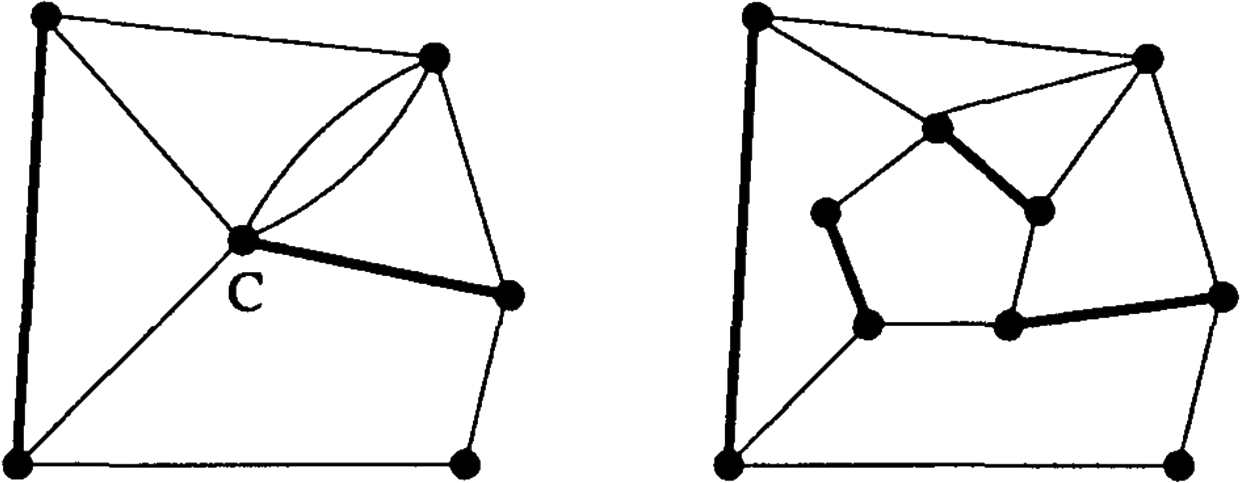
\includegraphics[width=0.5\textwidth]{extending}
		\caption{Extending}
	\end{figure}
\end{definition}
\begin{definition}[Ridurre e aggiornare un matching ed albero alternante]
	\textbf{Input:} Un matching \(M'\) del grafo \(G'\), un albero \(M'\)-alternante \(T\), ed un lato \(\rnd{v, w}\) di \(G'\) tale che \(v, w \in B\rnd{T}\).

	\textbf{Azione:} Sia \(C\) il circuito formato da \(\rnd{v, w}\) insieme con il cammino in \(T\) da \(v\) a \(w\). Aggiorniamo albero e matching come segue:
	\begin{align*}
		G'       & = G' \times C                 \\
		M'       & = M\setminus E\rnd{C}         \\
		E\rnd{T} & = E\rnd{T} \setminus E\rnd{C}
	\end{align*}
	\begin{figure}
		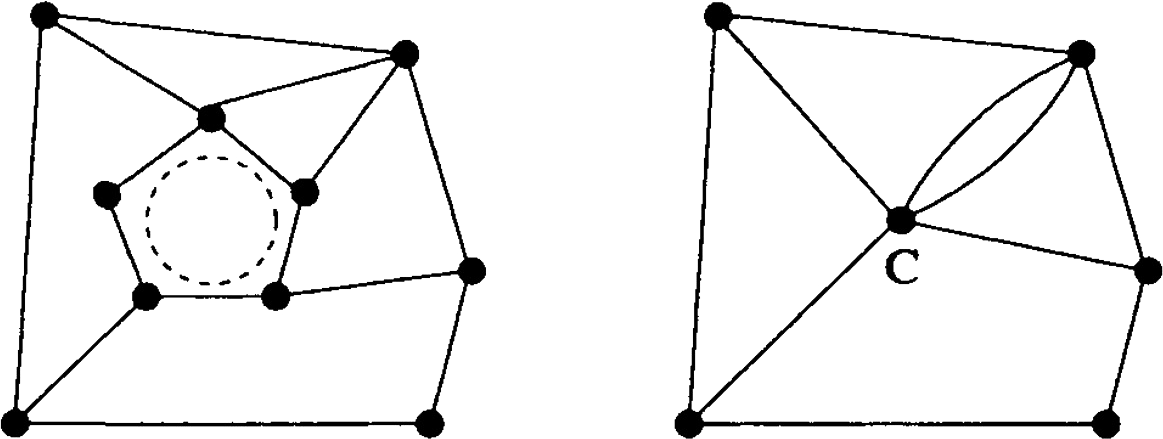
\includegraphics[width=0.5\textwidth]{schrinking}
		\caption{Shrinking}
	\end{figure}
\end{definition}
\clearpage
\begin{definition}[Aumentare un Matching]
	\textbf{Input:} Un matching \(M'\) di un grafo \(G'\), un albero \(M'\)-alternante \(T\) di \(G'\) con radice \(r\), un lato \(\rnd{v, w}\) di \(G'\) tale che \(v \in B\rnd{T}\), \(v \not\in V(T)\) e \(w\) sia \(M'\)-coperto.

	\textbf{Azione:} Sia \(P\) un cammino ottenuto appendendo \(\rnd{v, w}\) al cammino da \(r\) a \(v\) in \(T\). Il matching viene aggiornato come:
	\[
		M' = \crl{M'\cup E\rnd{P}}\setminus\crl{M' \cap E\rnd{P}}
	\]
\end{definition}
\begin{definition}[Albero alternante frustrato]
	Un albero alternante in un grafo \(\Gr \) si dice frustrato se ogni lato di \(G\) avente un termine in \(B(T)\) possiede l'altro termine in \(A(T)\).
\end{definition}
\begin{proposition}[Prima proposizione su AAF (5.6)]
	Sia \(\Gr \) un grafo con un matching \(M\) ed un albero alternante frustrato \(T\) associato ad esso. Allora \(G\) non possiede un matching perfetto.
\end{proposition}
\begin{proof}[Prima proposizione su AAF (5.6)]
	Ogni elemento di \(B(T)\) è una componente dispari a nodo singolo in \(G \setminus A(T)\).

	Siccome \(\abs{A(T)} < \abs{B(T)}\), per il teorema di Tutte \(G\) non possiede nessun matching perfetto.
\end{proof}
\begin{proposition}[Seconda proposizione su AAF (5.7)]
	Sia \(\Gr \) un grafo bipartito, \(M\) un matching definito su \(G\) e \(T\) un albero \(M\)-alternante tale che nessun lato di \(G\) sia posto tra un nodo in \(B(T)\) ed un nodo non in \(V(T)\). Allora risulta che \(T\) è frustrato e di conseguenza \(G\) non ha un matching perfetto.
\end{proposition}
\begin{proof}[Seconda proposizione su AAF (5.7)]
	Procediamo a mostrare che ogni lato avente un termine in \(B(T)\) possiede l'altro termine in \(A(T)\). Dalle ipotesi del teorema, l'unica possibile eccezione sarebbe un lato tra due nodi in \(B(T)\). Ma questo lato, insieme con i lati che lo uniscono alla radice \(r\), formerebbero un ciclo di lunghezza dispari, una cosa impossibile in un grafo bipartito.

	Di conseguenza \(T\) è frustrato e quindi per la prima proposizione su AAF (5.6), il grafo \(G\) non possiede un matching perfetto.
\end{proof}
\begin{definition}[Pseudonodo]
	In riferimento ad un grafo \(G'\) ottenuto da \(G\), vengono detti \textbf{pseudonodi} quei nodi che sono parte di \(G'\) ma non di \(G\).
\end{definition}
\begin{proposition}[Terza proposizione su AAF (5.8)]
	Sia \(G'\) un grafo derivato da \(G\), sia \(M'\) un matching di \(G'\) e sia \(T\) un albero \(M'\)-alternante frustrato di \(G'\) tale che nessun elemento di \(A(T)\) è uno pseudonodo.

	Se \(T\) è frustrato, allora \(G\) non possiede un matching perfetto.
\end{proposition}
\begin{proof}[Terza proposizione su AAF (5.8)]
	Se eliminassimo \(A(T)\) da \(G\) andremmo a ottenere una componente con un insieme di nodi \(S(v)\) per ogni nodo \(v \in B(T)\). Utilizzando quindi la formula di Tutte-Berge si ha che:
	\[
		\text{odd}\rnd{G \setminus A(T)} > \abs{A(T)}
	\]
	Ne segue che \(G\) non possiede un matching perfetto.
\end{proof}
\clearpage
\subsection{Diagramma della dimostrazione - Proposizioni sugli AAF}
\begin{figure}
	\includegraphics[width=\textwidth]{proofs/Proposizioni_sugli_AAF}
\end{figure}
\clearpage
\chapter{Algoritmo per il Matching Massimo}
Questo algoritmo identifica un cammino aumentante ed iniziando da un matching banale identifica un matching massimo in un dato grafo bipartito.

\section{Immagini step by step}
\begin{figure}
	\begin{subfigure}{0.5\textwidth}
		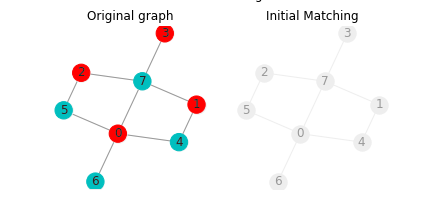
\includegraphics[width=\textwidth]{matching/0}
	\end{subfigure}
	\begin{subfigure}{0.25\textwidth}
		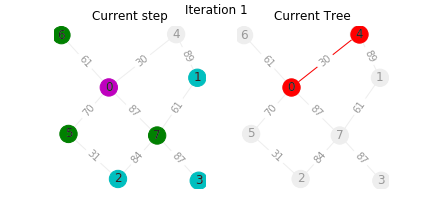
\includegraphics[width=\textwidth]{matching/1}
	\end{subfigure}
\end{figure}
\begin{figure}
	\begin{subfigure}{0.5\textwidth}
		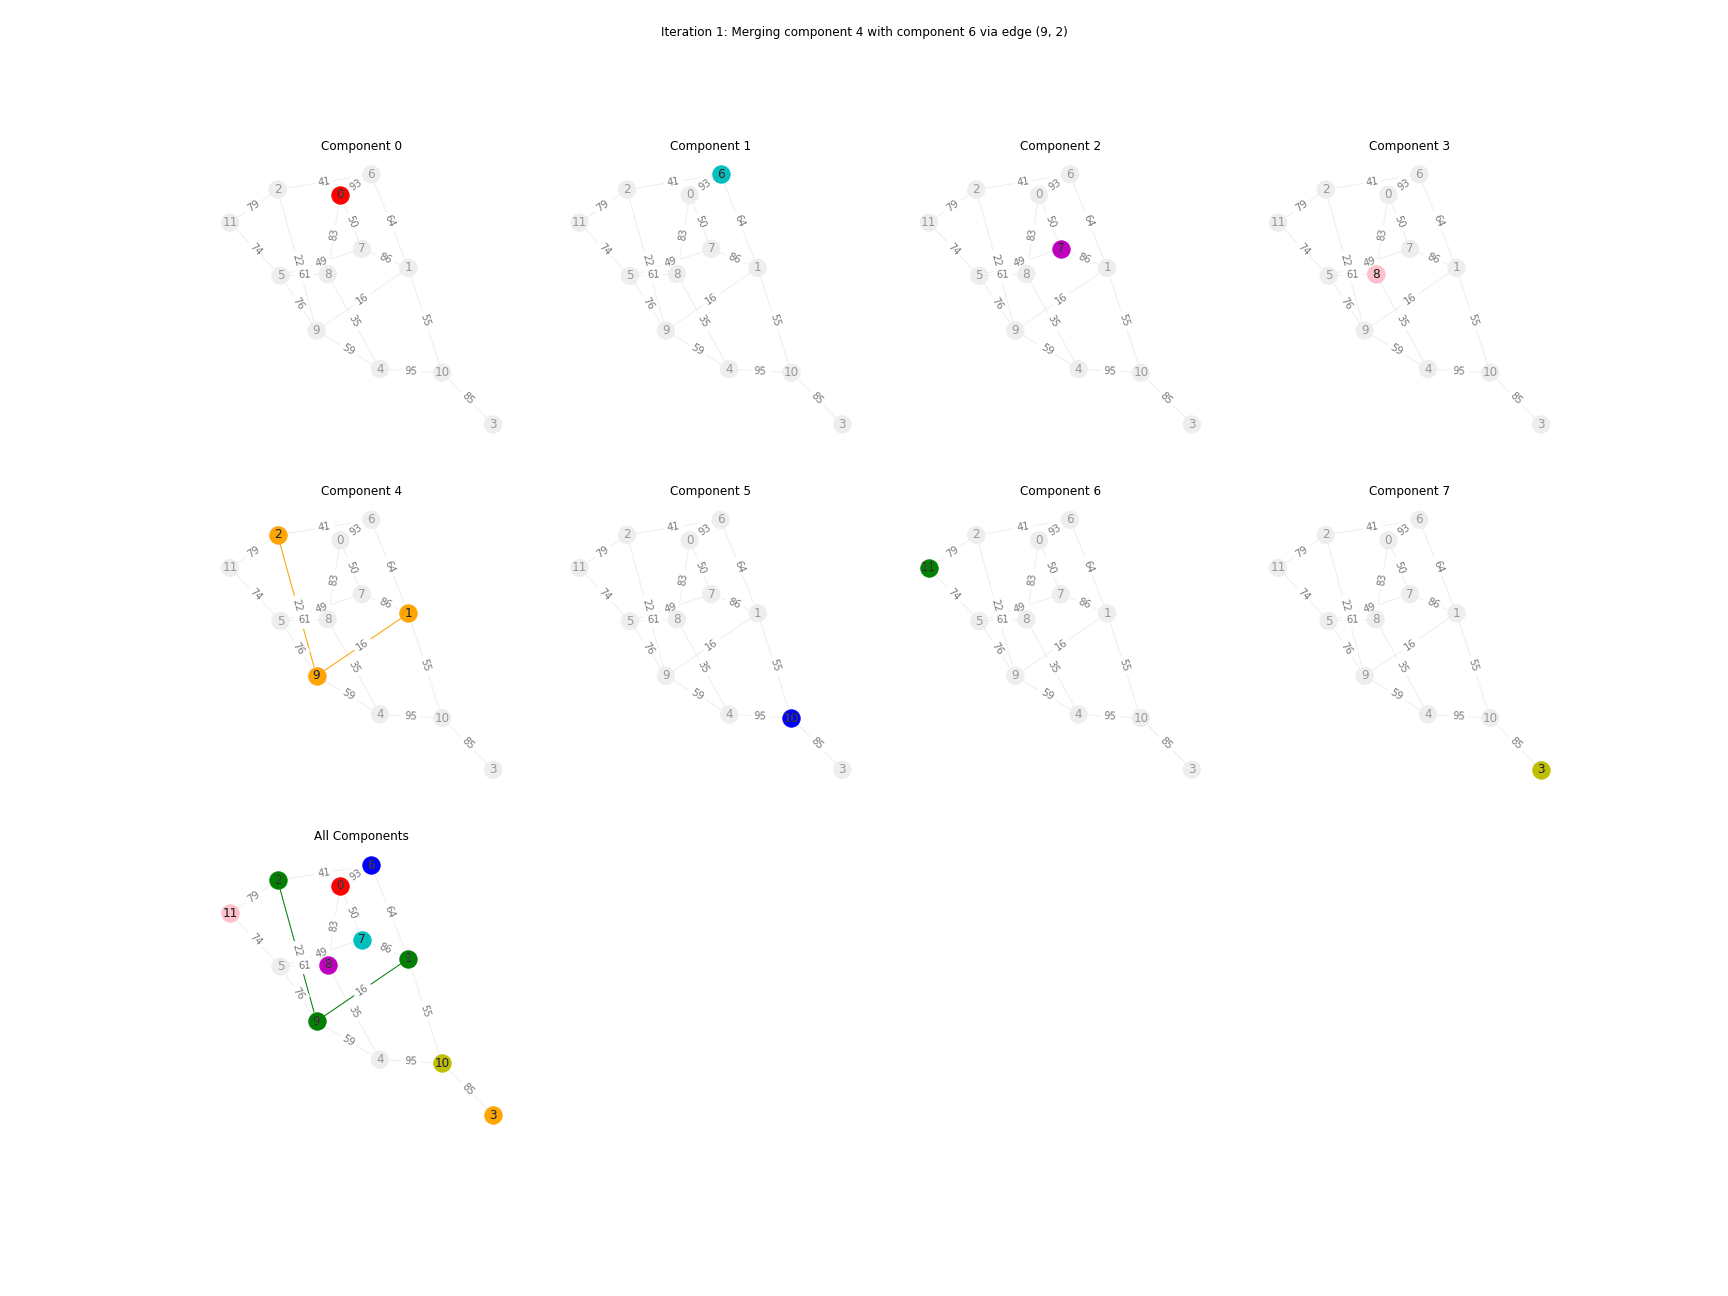
\includegraphics[width=\textwidth]{matching/2}
	\end{subfigure}
	\begin{subfigure}{0.5\textwidth}
		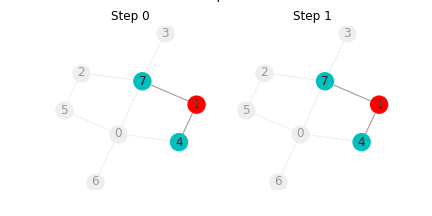
\includegraphics[width=\textwidth]{matching/3}
	\end{subfigure}
\end{figure}

\begin{figure}
	\begin{subfigure}{0.5\textwidth}
		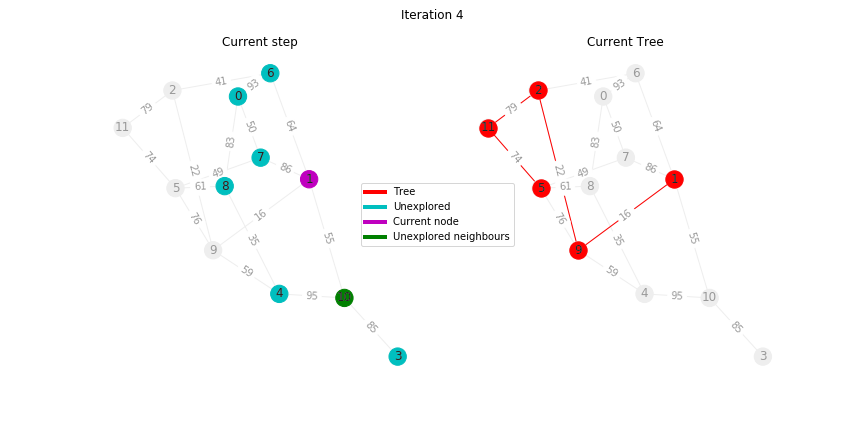
\includegraphics[width=\textwidth]{matching/4}
	\end{subfigure}
	\begin{subfigure}{0.25\textwidth}
		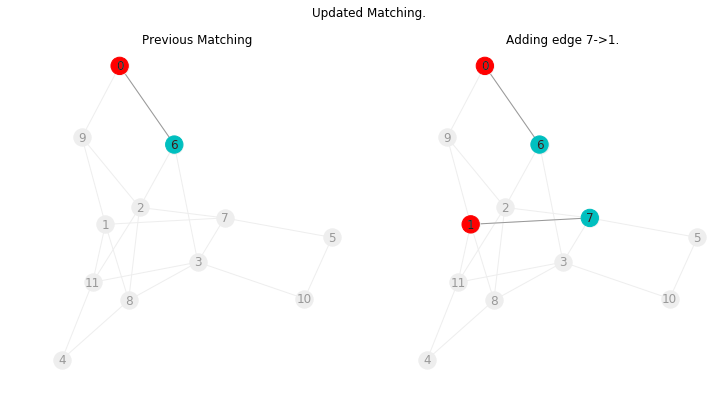
\includegraphics[width=\textwidth]{matching/5}
	\end{subfigure}
\end{figure}
\begin{figure}
	\begin{subfigure}{0.5\textwidth}
		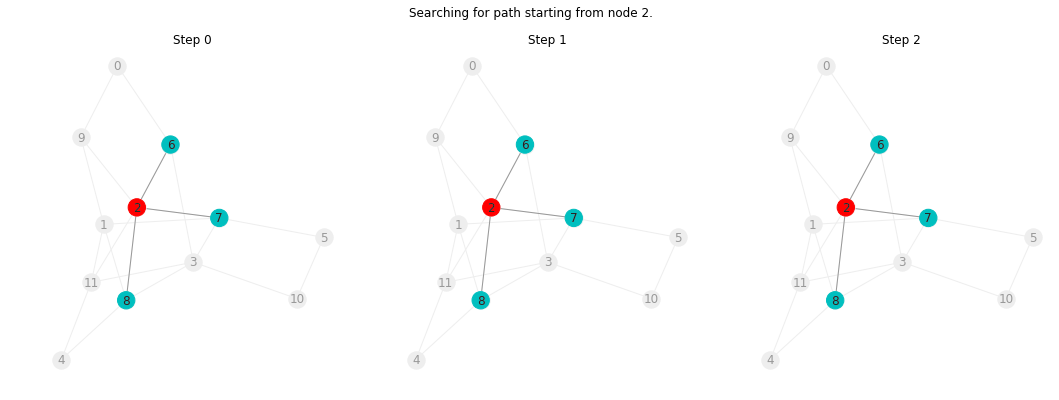
\includegraphics[width=\textwidth]{matching/6}
	\end{subfigure}
\end{figure}
\begin{figure}
	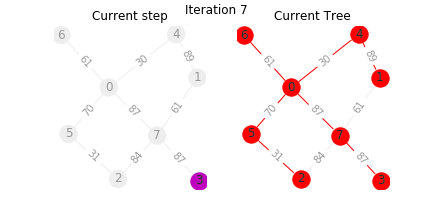
\includegraphics[width=\textwidth]{matching/7}
\end{figure}
\begin{figure}
	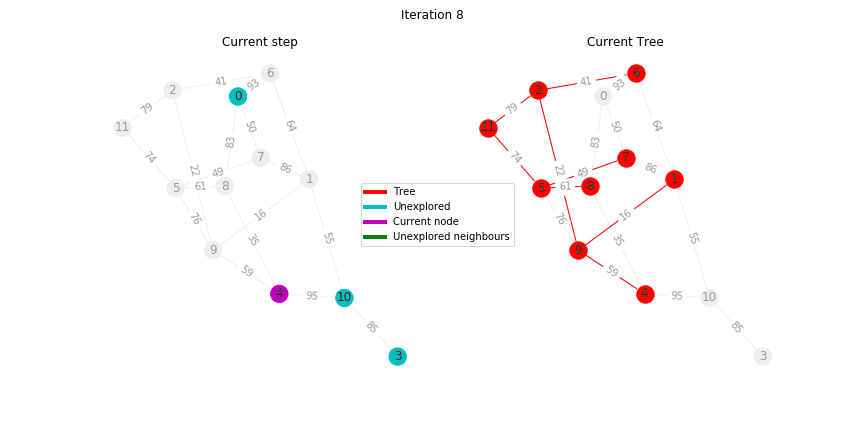
\includegraphics[width=\textwidth]{matching/8}
\end{figure}
\begin{figure}
	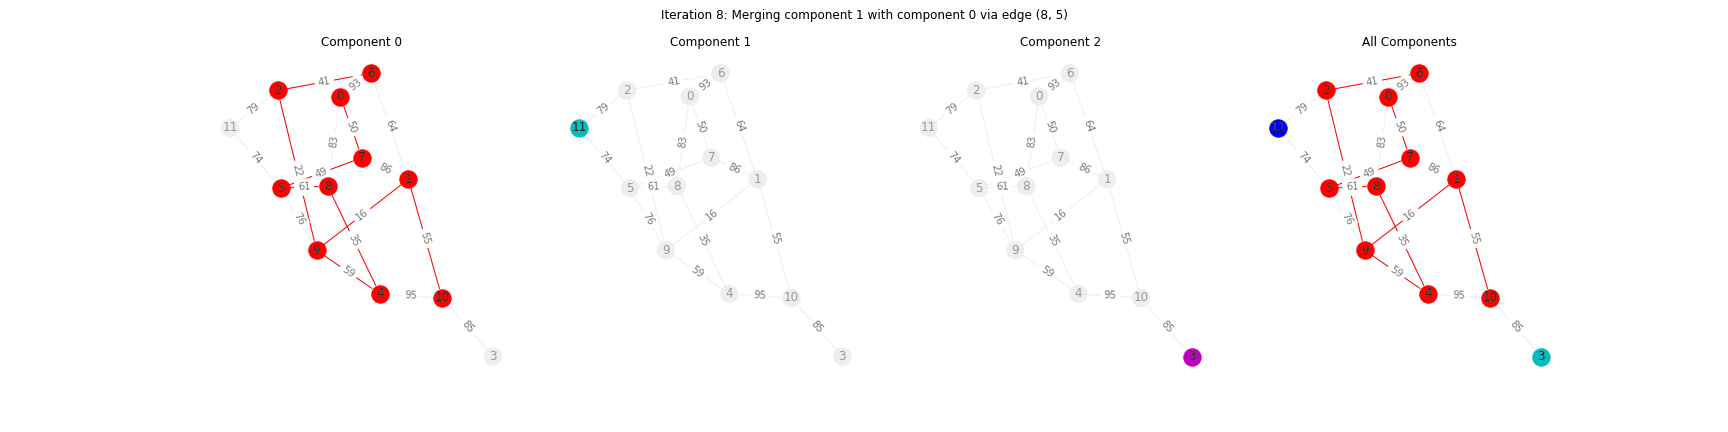
\includegraphics[width=0.75\textwidth]{matching/9}
\end{figure}

\clearpage
\section{Algoritmo Blossom}
L'algoritmo procede derivando grafi da un grafo bipartito \(G\) iniziale: se riesce ad identificare un matching perfetto in un grafo derivato allora è noto che esiste un matching perfetto in \(G\) e se riusciamo ad identificare un certo tipo di AAF all'interno di un grafo derivato possiamo concludere che \(G\) non possiede un matching perfetto. I grafi derivati \(G'\) vengono ottenuti identificando circuiti dispari all'interno dell'albero alternante \(T\) ottenuto da \(G\) e rimuovendoli attraverso un procedimento detto di ``shrinking'' (questo tipo di circuito veniva chiamato blossom, da cui il nome dell'algoritmo.)

\begin{theorem}[Algoritmo Blossom]
	L'algoritmo Blossom termina dopo \(\mathcal{O}(n)\) passi di ``augmentations'', \(\mathcal{O}(n^2)\) passi di ``shrinking'' e \(\mathcal{O}(n^2)\) passi di estensione dell'albero. Inoltre, determina correttamente se il grafo \(G\) possiede un matching perfetto.
\end{theorem}
\begin{proof}[Algoritmo Blossom]
	L'algoritmo inizia con un \textbf{matching} qualsiasi \(M=M'\) di \(G\), che non cessa di essere tale per tutto il procedimento.

	Siccome ad ogni passo di ``\textbf{augmentation}'' il numero di nodi esposti decresce, vi saranno \(\mathcal{O}(n)\) passi di ``\textbf{augmentation}''.

	Tra questi, ogni passo di ``\textbf{shrinking}'' riduce il numero dei nodi nel \textbf{grafo} \(G'\) senza tuttavia cambiare il numero dei nodi nell'\textbf{albero} \(T\) ed ogni passo di estensione dell'albero riduce il numero di nodi non in \(T\) non modificando il numero di nodi in \(G'\).

	Ne segue che il numero di passi di ``\textbf{shrinking}'' ed estensione dell'albero tra passi di ``\textbf{augmentation}'' è \(\mathcal{O}(n)\) e quindi in totale sono \(\mathcal{O}(n^2)\).

	Infine, siccome ogni \(G'\) è un grafo derivato da \(G\), se l'algoritmo termina con la conclusione che \(G'\) non possiede un matching perfetto, allora significa che ha trovato un albero con le proprietà descritte nella terza proposizione su AAF (5.8) e quindi \(G\) \textbf{non possiede un matching perfetto}.
\end{proof}
\clearpage
\subsection{Diagramma della dimostrazione - Algoritmo Blossom}
\begin{figure}
	\includegraphics[width=0.7\textwidth]{proofs/Algoritmo_Blossom}
\end{figure}
\clearpage
\section{Il postino cinese (Chinese postman problem, CPP)}
Sia \(\Gr \) un grafo connesso e sia \(w: E \rightarrow \R^+_0\) una lunghezza definita su \(G\). Vogliamo trovare un percorso chiuso \(C\) di lunghezza minima \(w(C)\) che contiene ogni lato di \(G\) almeno una volta.
\begin{definition}[Grafo e cammino euleriano]
	Un grafo è detto \textbf{euleriano} se è possibile tracciare un cammino che passa una sola volta per tutti gli archi del grafo. Un tale cammino è detto a sua volta euleriano.

	Equivalentemente, un grafo \(G\) è euleriano se e solo se ogni vertice ha grado pari e un cammino euleriano può essere costruiti con complessità \(\mathcal{O}(\abs{E})\).
\end{definition}
Se il grafo \(G\) risulta euleriano allora la soluzione del CPP è banale: qualsiasi cammino euleriano andrebbe bene.

Altrimenti si procede come segue: sia \(X\) l'insieme di tutti i vertici di \(G\) con grado dispari. Aggiungiamo un insieme di lati \(E'\) a \(G\) tale che le seguenti tre condizioni siano soddisfatte:
\begin{enumerate}
	\item Ogni lato \(e' \in E'\) è parallelo a qualche lato \(e \in E\). Estendiamo la distanza \(w\) a \(E'\) definendo \(w(e') = w(e)\).
	\item In \(V, E'\), solo i vertici di \(X\) hanno grado dispari.
	\item La distanza \(w(E')\) è minima: \(w(E') \leq w(E'')\) per ogni insieme \(E''\) che soddisfa le due condizioni precedenti.
\end{enumerate}
Ne segue che \(\rnd{V, E \cup E'}\) è un multigrafo euleriano, e ogni percorso euleriano introduce un cammino chiuso di lunghezza minima \(w(E) + w(E')\) in \(G\).

\subsection{Applicazione su grafo orientato}
\begin{definition}[Grafo orientato euleriano]
	Un grafo orientato è detto \textbf{euleriano} se tutti i vertici hanno grado entrante uguale al grado uscente.
\end{definition}
Consideriamo un grafo orientato non euleriano \(G\) e sia \(S(T)\) l'insieme di tutti i vertici che hanno un eccesso di archi entranti (o uscenti) rispetto a quelli uscenti (o entranti).

Indichiamo con \(d^{+(i)}\) (o \(d^{-(i)}\)) l'eccesso di grado entrante (o uscente) nei nodi di \(S(T)\). Per pareggiare il grado dei nodi \(i \in S(T)\) devo aggiungere \(d^{+(i)}\) (o \(d^{-(i)}\)) archi uscenti (o entranti). Poiché ogni arco contribuisce con un grado in uscita ed uno in ingresso, la somma totale dei gradi in uscita coincide con quella dei gradi in ingresso.

Come conseguenza la somma delle etichette \(d^{(i)}\) dei vertici in \(S\) coincide con quella dei vertici in \(T\). Calcolo il costo \(C_{ij}\) di un cammino di costo minimo fra ogni vertice \(i \in S\) ed ogni vertice \(j \in T\).

Costruisco una istanza di un problema di trasporto con gli insiemi \(S\) e \(T\), dove le quantità prodotte dai vertici in \(S\) e da trasportare a quelli in \(T\) sono le etichette \(d^{+(i)}\) mentre la domanda dei vertici in \(T\) sono i valori \(d^{-(i)}\), ed il costo per unità di merce trasportata lungo l'arco \((i,j)\) è \(C_{ij}\). La soluzione del problema di trasporto indica gli archi da aggiungere.

Se la soluzione dice di trasportare \(k\) unità di merda da \(i\) a \(j\) allora aggiungiamo \(k\) archi paralleli ad ogni arco nel cammino di costo minimo da \(i\) a \(j\).
\clearpage
\section{Algoritmi primali-duali}
Un algoritmo primale duale risolve problemi di programmazione lineare sfruttando la teoria della dualità e in particolare le condizioni di slackness complementare (o complementary slackness conditions, CSCs). L'algoritmo è inizializzato con una soluzione ammissibile nel problema duale e la corrispondente, in generale inammissibile, soluzione primale che soddisfino le CSCs.

Dopo ogni iterazione l'algoritmo mantiene una coppia della soluzione primale (inammissibile) e della soluzione duale (ammissibile), che soddisfino le CSCs.

L'algoritmo alterna le due iterazioni e riduce monotonamente l'inammissibilità primale fintanto che non raggiunge l'ammissibilità.

\paragraph*{Iterazione primale:} mantenendo la soluzione duale corrente fissata, si procede ad identificare una soluzione primale minimizzando l'inammissibilità primale tra le soluzioni ammissibili per le CSCs.
\paragraph*{Iterazione duale:} mantenendo fissata la soluzione primale corrente, si va a modificare la soluzione duale, mantenendola ammissibile e continuando a rispettare le CSCs.

\begin{definition}[Assegnamento parziale]
	Un \textbf{assegnamento parziale} è un assegnamento che rispetta i seguenti vincoli:
	\begin{align*}
		\sum_{j \in V_2} x_{ij} & \leq 1 \quad \forall i \in V_1 \\
		\sum_{i \in V_1} x_{ij} & \leq 1 \quad \forall j \in V_2
	\end{align*}
\end{definition}

\begin{definition}[Metrica di inammissibilità primale]
	Il valore dell'inammissibilità primale è determinato dal numero di assegnamenti mancanti.
\end{definition}

\begin{definition}[Cella ammissibile]
	Chiamiamo \textbf{cella ammissibile} della matrice ammissibile quelle per cui vale che:
	\[
		\bar{c}_{ij} = 0
	\]
\end{definition}

\clearpage
\chapter{Algoritmo Ungherese}
L'algoritmo ungherese (così chiamato perché basato sul lavoro di due matematici ungheresi), è un algoritmo primale-duale che serve ad identificare il matching di cardinalità massima e costo minimo in un grafo bipartito con matrice di incidenza pesata.

\section{Preprocessing}
\subsection{Bilanciamento del grafo}
Se il dato grafo bipartito non risultasse bilanciato, cioè \(\abs{V_1} \neq \abs{V_2}\), si procede a inserire vertici nella partizione di cardinalità minore fino che esse risultano bilanciate. Non aggiungendo lati, non vengono modificati i matching.

\subsection{Completare il grafo}
Se il grafo dato non fosse completo, cioè alcuni lati fossero assenti tra le due partizioni, si procede ad aggiungere lati con un costo molto alto in modo tale che essi non siano scelti, ma che in ogni caso il grafo risulti completo.

Questi nuovi lati portano alla creazione di matching nuovi, ma di costo estremamente alto.

\section{Il problema dell'assegnamento riformulato}
Possiamo quindi riformulare il problema come quello di trovare il matching completo tra due set di vertici in un dato grafo bipartito pesato: ogni soluzione è rappresentata da una \textbf{matrice di assegnamento}, una matrice quadrata dove un set rappresenta le righe e l'altro le colonne.

\section{Iterazione primale-duale}
\begin{figure}
	\begin{subfigure}{0.49\textwidth}
		\begin{align*}
			\min z = \sum_{i \in V_1} \sum_{j \in V_2} c_{ij}x_{ij}                    \\
			\sum_{j \in V_2}x_{ij} & = 1 \quad \forall i \in V_1                       \\
			\sum_{i \in V_1}x_{ij} & = 1 \quad \forall j \in V_2                       \\
			x_{ij}                 & \geq 0 \quad \forall i \in V_1, \forall j \in V_2
		\end{align*}
		\caption{Problema primale}
	\end{subfigure}
	\begin{subfigure}{0.49\textwidth}
		\begin{align*}
			\max w = \sum_{i\in V_1} u_i + \sum_{j \in V_2} v_j             \\
			u_i + v_j & \leq c_ij\quad \forall i \in V_1, \forall j \in V_2
		\end{align*}
		\caption{Problema duale}
	\end{subfigure}
\end{figure}
Le variabili duali \(\bmu \) e \(\bmv \) non sono vincolate in segno.

Le variabili di scarto complementare duale sono:
\[
	\bar{c} = c_{ij} - u_i - v_j
\]
Per garantire l'ottimalità della soluzione, le CSCs impongono che:
\[
	\bar{c}_{ij}x_{ij} = 0 \quad \forall i \in V_1, \forall j \in V_2
\]

\paragraph*{Iterazione primale} Mantenendo fissati \(\bmu \) e \(\bmv \) e mantenendo pertanto fissato anche \(\bbmc \) si procede a determinare una soluzione \(\bmx \) massimizzando il numero di assegnamenti (cioè di variabili unitarie) utilizzando solamente celle ammissibili.
\paragraph*{Iterazione duale} Si procede ad aggiornare \(\bmu \) e \(\bmv \), mantenendo \(\bar{c}_{ij}\) dove \(x_{ij} = 1\) e rendendo alcune celle ammissibili inammissibili.

\section{Pseudo codice}
\begin{figure}
	\begin{algorithm}[H]
		\SetAlgoLined
		Step 1: Inizializzazione duale di \(\bmu \) e \(\bmv \)\;
		Step 2: Inizializzazione primale di \(\bmx \)\;
		\While{\(\bmx \) è inammissibile}{
			Step 3.1: Inizializzazione del cammino\;
			\(Path \leftarrow nil\)\;
			\While{\(\rnd{Path = nil}\)}{
				\While{\(\rnd{Path = nil} \land \rnd{L \neq \emptyset}\)}{
					Step 3.2: Procedura di etichettatura\;
				}
				\If{\(Path = nil\)}{
					Step 4: Iterazione duale, modifica di \(\bmu \) e \(\bmv \)\;
				}
			}
			Step 5: Iterazione primale, modifica di \(\bmx \)\;
		}
		\caption{Algoritmo Ungherese}
	\end{algorithm}
\end{figure}

\section{Visualizzazione}

\begin{figure}
	\NewAdigraph{Hungarian}{
		s:0,0:\(s\);
		s1:2,2:\(s_1\);
		s2:2,0.75:\(s_2\);
		s3:2,-0.75:\(s_3\);
		s4:2,-2:\(s_4\);
		t1:5,2:\(t_1\);
		t2:5,0.75:\(t_2\);
		t3:5,-0.75:\(t_3\);
		t4:5,-2:\(t_4\);
		t:7,0:\(t\);
	}{
		s,s1;
		s,s2;
		s,s3;
		s,s4;
		t1,t;
		t2,t;
		t3,t;
		t4,t;
	}
	\Hungarian{}
	\caption{}
\end{figure}

\subsection{Primo step: Inizializzazione duale}

\begin{figure}
	\NewAdigraph{Hungarian}{
		s:0,0:\(s\);
		s1:2,2:\(s_1\);
		s2:2,0.75:\(s_2\);
		s3:2,-0.75:\(s_3\);
		s4:2,-2:\(s_4\);
		t1:5,2:\(t_1\);
		t2:5,0.75:\(t_2\);
		t3:5,-0.75:\(t_3\);
		t4:5,-2:\(t_4\);
		t:7,0:\(t\);
	}{
		s,s1;
		s,s2;
		s,s3;
		s,s4;
		t1,t;
		t2,t;
		t3,t;
		t4,t;
	}
	\Hungarian{}
	\caption{}
\end{figure}

\begin{figure}
	\NewAdigraph{Hungarian}{
		s:0,0:\(s\);
		s1:2,2:\(s_1\);
		s2:2,0.75:\(s_2\);
		s3:2,-0.75:\(s_3\);
		s4:2,-2:\(s_4\);
		t1:5,2:\(t_1\);
		t2:5,0.75:\(t_2\);
		t3:5,-0.75:\(t_3\);
		t4:5,-2:\(t_4\);
		t:7,0:\(t\);
	}{
		s,s1;
		s,s2;
		s,s3;
		s,s4;
		s1,t4;
		s2,t4;
		s3,t4;
		s4,t4;
		t1,t;
		t2,t;
		t3,t;
		t4,t;
	}
	\Hungarian{}
	\caption{}
\end{figure}

\NewAdigraph{DualInizializationLastStep}{
	s:0,0:\(s\);
	s1:2,2:\(s_1\);
	s2:2,0.75:\(s_2\);
	s3:2,-0.75:\(s_3\);
	s4:2,-2:\(s_4\);
	t1:5,2:\(t_1\);
	t2:5,0.75:\(t_2\);
	t3:5,-0.75:\(t_3\);
	t4:5,-2:\(t_4\);
	t:7,0:\(t\);
}{
	s,s1;
	s,s2;
	s,s3;
	s,s4;
	s1,t4;
	s2,t4;
	s3,t4;
	s4,t4;
	s4,t1;
	s4,t2;
	s4,t3;
	t1,t;
	t2,t;
	t3,t;
	t4,t;
}


\begin{figure}
	\DualInizializationLastStep{}
	\caption{}
\end{figure}

\subsection{Secondo step: Inizializzazione primale}

\begin{figure}
	\DualInizializationLastStep{}
	\caption{}
\end{figure}



\begin{figure}
	\NewAdigraph{Hungarian}{
		s:0,0:\(s\);
		s1:2,2:\(s_1\);
		s2:2,0.75:\(s_2\);
		s3:2,-0.75:\(s_3\);
		s4:2,-2:\(s_4\);
		t1:5,2:\(t_1\);
		t2:5,0.75:\(t_2\);
		t3:5,-0.75:\(t_3\);
		t4:5,-2:\(t_4\);
		t:7,0:\(t\);
	}{
		s,s2;
		s,s3;
		s,s4;
		s1,t4,red, 1;
		s2,t4;
		s3,t4;
		s4,t4;
		s4,t1;
		s4,t2;
		s4,t3;
		t2,t;
		t3,t;
		t4,t;
	}
	\Hungarian{}
	\caption{}
\end{figure}

\NewAdigraph{PrimalInitializationLastStep}{
	s:0,0:\(s\);
	s1:2,2:\(s_1\);
	s2:2,0.75:\(s_2\);
	s3:2,-0.75:\(s_3\);
	s4:2,-2:\(s_4\);
	t1:5,2:\(t_1\);
	t2:5,0.75:\(t_2\);
	t3:5,-0.75:\(t_3\);
	t4:5,-2:\(t_4\);
	t:7,0:\(t\);
}{
	s,s2;
	s,s3;
	s1,t4,red, 1;
	s2,t4;
	s3,t4;
	s4,t4;
	s4,t1,red,1;
	s4,t2;
	s4,t3;
	t2,t;
	t3,t;
}
\begin{figure}
	\PrimalInitializationLastStep{}
	\caption{}
\end{figure}

\subsection{Terzo step: Ricerca di un cammino aumentante}

\subsubsection{Step 3.1: Inizializzazione del cammino}

\begin{figure}
	\PrimalInitializationLastStep{}
	\caption{}
\end{figure}

\subsubsection{Step 3.2: Procedura di etichettatura}


\begin{figure}
	\NewAdigraph{Hungarian}{
		s:0,0:\(s\);
		s1:2,2:\(s_1\);
		s2,blue,1:2,0.75:\(s_2\);
		s3:2,-0.75:\(s_3\);
		s4:2,-2:\(s_4\);
		t1:5,2:\(t_1\);
		t2:5,0.75:\(t_2\);
		t3:5,-0.75:\(t_3\);
		t4,red,1:5,-2:\(t_4\);
		t:7,0:\(t\);
	}{
		s,s2;
		s,s3;
		s1,t4,red, 1;
		s2,t4;
		s3,t4;
		s4,t4;
		s4,t1,red,1;
		s4,t2;
		s4,t3;
		t2,t;
		t3,t;
	}
	\Hungarian{}
	\caption{}
\end{figure}

\begin{figure}
	\NewAdigraph{Hungarian}{
		s:0,0:\(s\);
		s1:2,2:\(s_1\);
		s2:2,0.75:\(s_2\);
		s3,blue,1:2,-0.75:\(s_3\);
		s4:2,-2:\(s_4\);
		t1:5,2:\(t_1\);
		t2:5,0.75:\(t_2\);
		t3:5,-0.75:\(t_3\);
		t4:5,-2:\(t_4\);
		t:7,0:\(t\);
	}{
		s,s2;
		s,s3;
		s1,t4,red, 1;
		s2,t4;
		s3,t4;
		s4,t4;
		s4,t1,red,1;
		s4,t2;
		s4,t3;
		t2,t;
		t3,t;
	}
	\Hungarian{}
	\caption{}
\end{figure}

\begin{figure}
	\NewAdigraph{Hungarian}{
		s:0,0:\(s\);
		s1,red,1:2,2:\(s_1\);
		s2:2,0.75:\(s_2\);
		s3:2,-0.75:\(s_3\);
		s4:2,-2:\(s_4\);
		t1:5,2:\(t_1\);
		t2:5,0.75:\(t_2\);
		t3:5,-0.75:\(t_3\);
		t4,blue,1:5,-2:\(t_4\);
		t:7,0:\(t\);
	}{
		s,s2;
		s,s3;
		s1,t4,red, 1;
		s2,t4;
		s3,t4;
		s4,t4;
		s4,t1,red,1;
		s4,t2;
		s4,t3;
		t2,t;
		t3,t;
	}
	\Hungarian{}
	\caption{}
\end{figure}

\begin{figure}
	\NewAdigraph{Hungarian}{
		s:0,0:\(s\);
		s1,blue,1:2,2:\(s_1\);
		s2:2,0.75:\(s_2\);
		s3:2,-0.75:\(s_3\);
		s4:2,-2:\(s_4\);
		t1:5,2:\(t_1\);
		t2:5,0.75:\(t_2\);
		t3:5,-0.75:\(t_3\);
		t4:5,-2:\(t_4\);
		t:7,0:\(t\);
	}{
		s,s2;
		s,s3;
		s1,t4,red, 1;
		s2,t4;
		s3,t4;
		s4,t4;
		s4,t1,red,1;
		s4,t2;
		s4,t3;
		t2,t;
		t3,t;
	}
	\Hungarian{}
	\caption{}
\end{figure}

\subsection{Step 4: Iterazione duale}

\begin{figure}
	\NewAdigraph{Hungarian}{
		s:0,0:\(s\);
		s1:2,2:\(s_1\);
		s2:2,0.75:\(s_2\);
		s3:2,-0.75:\(s_3\);
		s4:2,-2:\(s_4\);
		t1:5,2:\(t_1\);
		t2:5,0.75:\(t_2\);
		t3:5,-0.75:\(t_3\);
		t4:5,-2:\(t_4\);
		t:7,0:\(t\);
	}{
		s,s2;
		s,s3;
		s1,t4,red, 1;
		s2,t4;
		s3,t4;
		s4,t4;
		s4,t1,red,1;
		s4,t2;
		s4,t3;
		t2,t;
		t3,t;
	}
	\Hungarian{}
	\caption{}
\end{figure}

\begin{figure}
	\NewAdigraph{Hungarian}{
		s:0,0:\(s\);
		s1:2,2:\(s_1\);
		s2:2,0.75:\(s_2\);
		s3:2,-0.75:\(s_3\);
		s4:2,-2:\(s_4\);
		t1,red,1:5,2:\(t_1\);
		t2:5,0.75:\(t_2\);
		t3:5,-0.75:\(t_3\);
		t4:5,-2:\(t_4\);
		t:7,0:\(t\);
	}{
		s,s2;
		s,s3;
		s1,t4,red, 1;
		s2,t4;
		s2,t1,blue,1;
		s3,t4;
		s4,t4,gray,0.2;
		s4,t1,red,1;
		s4,t2;
		s4,t3;
		t2,t;
		t3,t;
	}
	\Hungarian{}
	\caption{}
\end{figure}

\begin{figure}
	\NewAdigraph{Hungarian}{
		s:0,0:\(s\);
		s1:2,2:\(s_1\);
		s2:2,0.75:\(s_2\);
		s3:2,-0.75:\(s_3\);
		s4,red,1:2,-2:\(s_4\);
		t1,blue,1:5,2:\(t_1\);
		t2:5,0.75:\(t_2\);
		t3:5,-0.75:\(t_3\);
		t4:5,-2:\(t_4\);
		t:7,0:\(t\);
	}{
		s,s2;
		s,s3;
		s1,t4,red, 1;
		s2,t4;
		s2,t1;
		s3,t4;
		s4,t1,red,1;
		s4,t2;
		s4,t3;
		t2,t;
		t3,t;
	}
	\Hungarian{}
	\caption{}
\end{figure}

\begin{figure}
	\NewAdigraph{Hungarian}{
		s:0,0:\(s\);
		s1:2,2:\(s_1\);
		s2:2,0.75:\(s_2\);
		s3:2,-0.75:\(s_3\);
		s4,blue,1:2,-2:\(s_4\);
		t1:5,2:\(t_1\);
		t2,red,1:5,0.75:\(t_2\);
		t3,red,1:5,-0.75:\(t_3\);
		t4:5,-2:\(t_4\);
		t:7,0:\(t\);
	}{
		s,s2;
		s,s3;
		s1,t4,red, 1;
		s2,t4;
		s2,t1;
		s3,t4;
		s4,t1,red,1;
		s4,t2;
		s4,t3;
		t2,t;
		t3,t;
	}
	\Hungarian{}
	\caption{}
\end{figure}

\begin{figure}
	\NewAdigraph{Hungarian}{
		s:0,0:\(s\);
		s1:2,2:\(s_1\);
		s2:2,0.75:\(s_2\);
		s3:2,-0.75:\(s_3\);
		s4:2,-2:\(s_4\);
		t1:5,2:\(t_1\);
		t2,blue,1:5,0.75:\(t_2\);
		t3:5,-0.75:\(t_3\);
		t4:5,-2:\(t_4\);
		t:7,0:\(t\);
	}{
		s,s2,,2;
		s,s3;
		s1,t4,red, 1;
		s2,t4;
		s2,t1,,2;
		s3,t4;
		s4,t1,red,2;
		s4,t2,,2;
		s4,t3;
		t2,t,,2;
		t3,t;
	}
	\Hungarian{}
	\caption{}
\end{figure}

\subsection{Step 5: Iterazione primale}

\begin{figure}
	\NewAdigraph{Hungarian}{
		s:0,0:\(s\);
		s1:2,2:\(s_1\);
		s2:2,0.75:\(s_2\);
		s3:2,-0.75:\(s_3\);
		s4,red,1:2,-2:\(s_4\);
		t1:5,2:\(t_1\);
		t2,blue,1:5,0.75:\(t_2\);
		t3:5,-0.75:\(t_3\);
		t4:5,-2:\(t_4\);
		t:7,0:\(t\);
	}{
		s,s2;
		s,s3;
		s1,t4,red, 1;
		s2,t4;
		s2,t1;
		s3,t4;
		s4,t1,red,1;
		s4,t2,red,1;
		s4,t3;
		t2,t;
		t3,t;
	}
	\Hungarian{}
	\caption{}
\end{figure}

\begin{figure}
	\NewAdigraph{Hungarian}{
		s:0,0:\(s\);
		s1:2,2:\(s_1\);
		s2:2,0.75:\(s_2\);
		s3:2,-0.75:\(s_3\);
		s4,blue,1:2,-2:\(s_4\);
		t1,red,1:5,2:\(t_1\);
		t2:5,0.75:\(t_2\);
		t3:5,-0.75:\(t_3\);
		t4:5,-2:\(t_4\);
		t:7,0:\(t\);
	}{
		s,s2;
		s,s3;
		s1,t4,red, 1;
		s2,t4;
		s2,t1;
		s3,t4;
		s4,t1;
		s4,t2,red,1;
		s4,t3;
		t2,t;
		t3,t;
	}
	\Hungarian{}
	\caption{}
\end{figure}

\begin{figure}
	\NewAdigraph{Hungarian}{
		s:0,0:\(s\);
		s1:2,2:\(s_1\);
		s2,red,1:2,0.75:\(s_2\);
		s3:2,-0.75:\(s_3\);
		s4:2,-2:\(s_4\);
		t1,blue,1:5,2:\(t_1\);
		t2:5,0.75:\(t_2\);
		t3:5,-0.75:\(t_3\);
		t4:5,-2:\(t_4\);
		t:7,0:\(t\);
	}{
		s,s2;
		s,s3;
		s1,t4,red, 1;
		s2,t4;
		s2,t1;
		s3,t4;
		s4,t1;
		s4,t2,red,1;
		s4,t3;
		t2,t;
		t3,t;
	}
	\Hungarian{}
	\caption{}
\end{figure}

\begin{figure}
	\NewAdigraph{Hungarian}{
		s,red,1:0,0:\(s\);
		s1:2,2:\(s_1\);
		s2,blue,1:2,0.75:\(s_2\);
		s3:2,-0.75:\(s_3\);
		s4:2,-2:\(s_4\);
		t1,blue,1:5,2:\(t_1\);
		t2:5,0.75:\(t_2\);
		t3:5,-0.75:\(t_3\);
		t4:5,-2:\(t_4\);
		t:7,0:\(t\);
	}{
		s,s2,gray,0.2;
		s,s3;
		s1,t4,red, 1;
		s2,t4;
		s2,t1;
		s3,t4;
		s4,t1;
		s4,t2,red,1;
		s4,t3;
		t2,t;
		t3,t;
	}
	\Hungarian{}
	\caption{}
\end{figure}



\end{document}